% Sprache für das Dokument festlegen
\newcommand{\frauassprache}{en} % de oder en für Deutsch oder Englisch

% Dokumententyp und benutzte Pakete
\documentclass[open=right,  % Kapitel darf nur auf rechten Seite beginnen
    paper=a4,               % DIN-A4-Papier
    fontsize=11pt,          % Schriftgöße
    headings=small,         % Kleine Überschriften
    headsepline=true,       % Trennlinie am Kopf der Seite
    footsepline=false,      % Keine Trennlinie am Fuß der Seite
    bibliography=totoc,     % Literaturverzeichnis in das Inhaltsverzeichnis aufnehmen
    twoside=true,             % Doppelseitiger Druck - auf off stellen für einseitig
    DIV=7,                  % Verhältnis der Ränder zum bedruckten Bereich
    chapterprefix=true,     % Kapitel x vor dem Kapitelnamen
    cleardoublepage=plain]{scrbook}

% Pakete einbinden, die benötigt werden
\usepackage{ifthen}               % Logische Bedingungen mit ifthenelse
\usepackage{scrlayer-scrpage}     % Erweiterte Einstellungen an scrbook zulassen
\usepackage[utf8]{inputenc}       % Dateien in UTF-8 benutzen
\usepackage[T1]{fontenc}          % Zeichenkodierung
\usepackage{graphicx}             % Bilder einbinden
\usepackage{enumitem}             % Eigene Listen definieren können
\usepackage{setspace}             % Abstände korrigieren

% Setzen von Optionen abhängig von der gewählten Sprache. Die Sprache wird
% in thesis.tex gesetzt.
\ifthenelse{\equal{\frauassprache}{de}}%
{%
 \usepackage[main=ngerman, english]{babel}  % Deutsche Sprachunterstützung
 \usepackage[autostyle=true,german=quotes]{csquotes} % Deutsche Anführungszeichen
 \usepackage[pagebackref=false,german]{hyperref} % Hyperlinks
 \newcommand{\frauassortlocale}{de_DE} % Sortierung der Literatur
}%
{%
 \usepackage[main=english, ngerman]{babel} % Englische Sprachunterstützung
 \usepackage[autostyle=true,english=american]{csquotes} % Englische Anführungszeichen
 \usepackage[pagebackref=false,english]{hyperref}  % Hyperlinks
 \newcommand{\frauassortlocale}{en_US} % Sortierung der Literatur
}%

\usepackage{xcolor}               % Unterstützung für Farben
\usepackage{amsmath}              % Mathematische Formeln
\usepackage{amsfonts}             % Mathematische Zeichensätze
\usepackage{amssymb}              % Mathematische Symbole
\usepackage{float}                % Fließende Objekte (Tabellen, Grafiken etc.)
\usepackage{booktabs}             % Korrekter Tabellensatz
\usepackage[printonlyused]{acronym}  % Abkürzungsverzeichnis [nur verwendete Abkürzungen]
\usepackage{makeidx}              % Sachregister
\usepackage{listings}             % Quelltexte
\usepackage{listingsutf8}         % Quelltexte in UTF8
\usepackage[hang,font={sf,footnotesize},labelfont={footnotesize,bf}]{caption} % Beschriftungen
\usepackage[scaled]{helvet}       % Schrift Helvetia laden
\usepackage[absolute]{textpos}    % Absolute Textpositionen (für Deckblatt)
\usepackage{calc}                 % Berechnung von Positionen
\usepackage{blindtext}            % Blindtexte
%\usepackage[bottom=40mm,left=30mm,right=30mm,top=35mm]{geometry} % Ränder ändern
\usepackage[ 											% Ränder ändern
	a4paper, 
	showframe=false,
	textwidth=420pt,
	textheight=620pt,
	footskip=40pt,
]{geometry}
\usepackage{scrhack}              % tocbasic Warnung entfernen
\usepackage[all]{hypcap}          % Korrekte Verlinkung von Floats
\usepackage{tabularx}             % Spezielle Tabellen
\usepackage[
  backend       = bibtex8, %minalphanames only works with biber backend
  bibstyle      = numeric-comp,
  citestyle     = numeric-comp,
  firstinits    = true,
  useprefix     = true, %print "von, van, etc.", too.
  minnames      = 1,
  minalphanames = 3,
  maxalphanames = 4,
  maxbibnames   = 99,
  maxcitenames  = 3,
	url						= false,
  doi           = true, %source: http://tex.stackexchange.com/a/23118/9075
  isbn          = true, %source: http://tex.stackexchange.com/a/23118/9075
	eprint				= false,
  backref       = true]{biblatex}
\usepackage{rotating}             % Seiten drehen
\usepackage{harveyballs}          % Harveyballs
\usepackage{chngcntr}             % Counter (Zähler) ändern können - für Fußnotennummern

% Einstellungen zu den Fußnoten
\renewcommand{\footnotesize}{\fontsize{9}{10}\selectfont} % Größe der Fußnoten
\setlength{\footnotesep}{8pt} % Abstand zwischen den Fußnoten

% Kommentieren Sie diese Zeile ein, wenn Sie eine "durchlaufende" Nummerierung bei den
% Fußnoten wünschen, d.h. wenn die Fußnoten nicht bei jedem Kapitel wieder bei 1
% beginnen sollen.
%\counterwithout{footnote}{chapter}

\setlength{\bibitemsep}{1em}      % Abstand zwischen den Literaturangaben
\setlength{\bibhang}{2em}         % Einzug nach jeweils erster Zeile

% Trennung von URLs im Literaturverzeichnis (große Werte [> 10000] verhindern die Trennung)
\defcounter{biburlnumpenalty}{10} % Strafe für Trennung in URL nach Zahl
\defcounter{biburlucpenalty}{500} % Strafe für Trennung in URL nach Großbuchstaben
\defcounter{biburllcpenalty}{500} % Strafe für Trennung in URL nach Kleinbuchstaben

% Farben definieren
\definecolor{linkblue}{RGB}{0, 0, 100}
\definecolor{linkblack}{RGB}{0, 0, 0}
\definecolor{comment}{RGB}{63, 127, 95}
\definecolor{darkgreen}{RGB}{14, 144, 102}
\definecolor{darkblue}{RGB}{0,0,168}
\definecolor{darkred}{RGB}{128,0,0}
\definecolor{javadoccomment}{RGB}{0,0,240}

% Einstellungen für das Hyperlink-Paket
\hypersetup{
    colorlinks=true,      % Farbige links verwenden
%    allcolors=linkblue,
    linktoc=all,          % Links im Inhaltsverzeichnis
    linkcolor=linkblack,  % Querverweise
    citecolor=linkblack,  % Literaturangaben
    filecolor=linkblack,  % Dateilinks
    urlcolor=linkblack    % URLs
}

% Einstellungen für Quelltexte
\lstset{
      xleftmargin=0.2cm,
      basicstyle=\footnotesize\ttfamily,
      keywordstyle=\color{darkgreen},
      identifierstyle=\color{darkblue},
      commentstyle=\color{comment},
      stringstyle=\color{darkred},
      tabsize=2,
      lineskip={2pt},
      columns=flexible,
      inputencoding=utf8,
      captionpos=b,
      breakautoindent=true,
      breakindent=2em,
      breaklines=true,
      prebreak=,
      postbreak=,
      numbers=none,
      numberstyle=\tiny,
      showspaces=false,      % Keine Leerzeichensymbole
      showtabs=false,        % Keine Tabsymbole
      showstringspaces=false,% Leerzeichen in Strings
      morecomment=[s][\color{javadoccomment}]{/**}{*/},
      literate={Ö}{{\"O}}1 {Ä}{{\"A}}1 {Ü}{{\"U}}1 {ß}{{\ss}}2 {ü}{{\"u}}1 {ä}{{\"a}}1 {ö}{{\"o}}1
}

\urlstyle{same}

% Einstellungen für Überschriften
\renewcommand*{\chapterformat}{%
  \LARGE\chapapp~\thechapter
  \vspace{0.3cm}
} 
% Abstände für die Überschriften setzen
\renewcommand{\chapterheadstartvskip}{\vspace*{2.6cm}}
\renewcommand{\chapterheadendvskip}{\vspace*{1.5cm}}

% Vertikale Abstände für die Überschriften etwas verkleinern
\RedeclareSectionCommand[
  beforeskip=-1.0\baselineskip,
  afterskip=0.25\baselineskip]{section}

\RedeclareSectionCommand[
  beforeskip=-1.0\baselineskip,
  afterskip=0.15\baselineskip]{subsection}

\RedeclareSectionCommand[
  beforeskip=-1.0\baselineskip,
  afterskip=0.15\baselineskip]{subsubsection}

% In der Kopfzeile nur die kurze Kapitelbezeichnung (ohne Kapitel davor)
\renewcommand*\chaptermarkformat{\thechapter\autodot\enskip}
\automark[chapter]{chapter}

% Einstellungen für Schriftarten
\setkomafont{pagehead}{\normalfont\sffamily}
\setkomafont{pagenumber}{\normalfont\sffamily}
\setkomafont{paragraph}{\sffamily\bfseries\small}
\setkomafont{subsubsection}{\sffamily\itshape\bfseries\small}
\addtokomafont{footnote}{\sffamily\footnotesize\sffamily}
\setkomafont{chapter}{\Huge\selectfont\bfseries}
\renewcommand*{\bibfont}{\normalsize\sffamily}

% Wichtige Abstände
\setlength{\parskip}{0.0cm}  % 2mm Abstand zwischen zwei Absätzen
\setlength{\parindent}{1.5em}  % Absätze nicht einziehen
\clubpenalty = 10000         % Keine "Schusterjungen"
\widowpenalty = 10000        % Keine "Hurenkinder"
\displaywidowpenalty = 10000 % Keine "Hurenkinder"
                             % Siehe: https://de.wikipedia.org/wiki/Hurenkind_und_Schusterjunge
\pdfminorversion=5 
\pdfcompresslevel=9
\pdfobjcompresslevel=2

% Index erzeugen
\makeindex

% Einfacher Font-Wechsel über dieses Makro
\newcommand{\changefont}[3]{
\fontfamily{#1} \fontseries{#2} \fontshape{#3} \selectfont}

% Eigenes Makro für Bilder. Das label (für \ref) ist dann einfach
% der Name der Bilddatei
\newcommand{\bild}[3]{
\begin{figure}[ht]
  \centering
  \includegraphics[width=#2]{#1}
  \caption{#3}
  \label{#1}
\end{figure}}

% Wo liegt Sourcecode?
\newcommand{\srcloc}{src/}

% Wo sind die Bilder?
\graphicspath{{bilder/}}

% Makros für typographisch korrekte Abkürzungen
\newcommand{\zb}[0]{z.\,B.}
\newcommand{\dahe}[0]{d.\,h.}
\newcommand{\ua}[0]{u.\,a.}

% Flags für Veröffentlichung und Sperrvermerk
\newboolean{frauaspublizieren}
\newboolean{frauassperrvermerk}

% Tabellenzellen mit mehreren Zeilen
\newcolumntype{L}{>{\raggedright\arraybackslash}X}
\newcolumntype{b}{l}
\newcolumntype{s}{>{\hsize=.3\hsize}l}
\newcolumntype{F}{>{\hsize=\dimexpr2\hsize+2\tabcolsep+\arrayrulewidth\relax}X}

% Checklisten mit zwei Ebenen
\newlist{checklist}{itemize}{2}
\setlist[checklist]{label=$\square$}

% Dokumenteninfos importieren
% -------------------------------------------------------
% Daten für die Arbeit
% Wenn hier alles korrekt eingetragen wurde, wird das Titelblatt
% automatisch generiert. D.h. die Datei titelblatt.tex muss nicht mehr
% angepasst werden.

% Titel der Arbeit auf Deutsch
\newcommand{\frauastitelde}{Einsatz eines Flux-Kompensators für Zeitreisen mit einer maximalen Höchstgeschwindigkeit von WARP~7}

% Titel der Arbeit auf Englisch
\newcommand{\frauastitelen}{Application of a Flux Compensator for Timetravel with a Maximum Velocity of Warp~7}

% Weitere Informationen zur Arbeit
\newcommand{\frauasort}{Frankfurt am Main}    % Ort
\newcommand{\frauasautorvname}{Max} % Vorname(n)
\newcommand{\frauasautornname}{Mustermann} % Nachname(n)
\newcommand{\frauasdatum}{24.10.2019} % Datum der Abgabe
\newcommand{\frauasjahr}{2019} % Jahr der Abgabe
\newcommand{\frauasfirma}{Paukenschlag GmbH, Frankfurt am Main} % Firma bei der die Arbeit durchgeführt wurde
\newcommand{\frauasbetreuer}{Prof. Peter Mustermann, University of Applied Sciences} % Betreuer an der Hochschule
\newcommand{\frauaszweitkorrektor}{Erika Mustermann, Paukenschlag GmbH} % Betreuer im Unternehmen oder Zweitkorrektor
\newcommand{\frauasfakultaet}{I} % I für Informatik oder E, S, B, D, M, N, W, V
\newcommand{\frauasstudiengang}{IB} % IB IMB UIB CSB IM MTB (weitere siehe titleblatt.tex)

% Zustimmung zur Veröffentlichung
\setboolean{frauaspublizieren}{true}   % Einer Veröffentlichung wird zugestimmt
\setboolean{frauassperrvermerk}{false} % Die Arbeit hat keinen Sperrvermerk

% -------------------------------------------------------
% Abstract
% Achtung: Wenn Sie im Abstrakt Anführungszeichen verwenden wollen, dann benutzen Sie
%          nicht "` und "', sondern \enquote{}. "` und "' werden nicht richtig
%          erkannt.

% Kurze (maximal halbseitige) Beschreibung, worum es in der Arbeit geht auf Deutsch
\newcommand{\frauasabstractde}{Jemand musste Josef K. verleumdet haben, denn ohne dass er etwas Böses getan hätte, wurde er eines Morgens verhaftet. Wie ein Hund! sagte er, es war, als sollte die Scham ihn überleben. Als Gregor Samsa eines Morgens aus unruhigen Träumen erwachte, fand er sich in seinem Bett zu einem ungeheueren Ungeziefer verwandelt. Und es war ihnen wie eine Bestätigung ihrer neuen Träume und guten Absichten, als am Ziele ihrer Fahrt die Tochter als erste sich erhob und ihren jungen Körper dehnte. Es ist ein eigentümlicher Apparat, sagte der Offizier zu dem Forschungsreisenden und überblickte mit einem gewissermaßen bewundernden Blick den ihm doch wohl bekannten Apparat. Sie hätten noch ins Boot springen können, aber der Reisende hob ein schweres, geknotetes Tau vom Boden, drohte ihnen damit und hielt sie dadurch von dem Sprunge ab. In den letzten Jahrzehnten ist das Interesse an Künstlern sehr zurückgegangen. Aber sie überwanden sich, umdrängten den Käfig und wollten sich gar nicht fortrühren.}

% Kurze (maximal halbseitige) Beschreibung, worum es in der Arbeit geht auf Englisch
\newcommand{\frauasabstracten}{The European languages are members of the same family. Their separate existence is a myth. For science, music, sport, etc, Europe uses the same vocabulary. The languages only differ in their grammar, their pronunciation and their most common words. Everyone realizes why a new common language would be desirable: one could refuse to pay expensive translators. To achieve this, it would be necessary to have uniform grammar, pronunciation and more common words. If several languages coalesce, the grammar of the resulting language is more simple and regular than that of the individual languages. The new common language will be more simple and regular than the existing European languages. It will be as simple as Occidental; in fact, it will be Occidental. To an English person, it will seem like simplified English, as a skeptical Cambridge friend of mine told me what Occidental is.}


% Literatur-Datenbank
\bibliography{bibliography}
%\addbibresource{bibliography.bib}   % BibLaTeX-Datei mit Literaturquellen einbinden
\hyphenation{
multi-screen
}

% Anfang des Dokuments
\begin{document}
% Die Seitennummerierung erfolgt durchlaufend ab der Titelseite. Also keine
% Spielereien mit römischen Ziffern usw. - Die ISO 7144 schreibt das sogar für
% wissenschaftliche Werke vor.
% Von Promitionsordnung verlangt!
% Deshalb ist \frontmatter DEAKTIVIERT

% Römische Ziffern für die "Front-Matter"
\setcounter{page}{0}
%\changefont{ptm}{m}{n}  % Times New Roman für den Fließtext
%\renewcommand{\rmdefault}{ptm}

% Titelblatt
% *******************************************************************
% In dieser Datei sollten eigentlich keine Veränderungen
% notwendig sein. Alle Einstellungen erfolgen in docinfo.tex und
% der thesis.tex.
% *******************************************************************

\thispagestyle{empty}

% Fakultäten 
% *******************************************************************
\ifthenelse{\equal{\frauasfakultaet}{I}}%
  {\newcommand{\frauasfakultaetlangde}{Fachbereichs Informatik und Ingenieurwissenschaften}%
   \newcommand{\frauasfakultaetlangen}{Faculty of Computer Science and Engineering}}{} 

% Studiengänge 
% *******************************************************************
\ifthenelse{\equal{\frauasstudiengang}{IB}}%
  {\newcommand{\frauasstudienganglangde}{Informatik}%
  \newcommand{\frauasstudienganglangen}{Computer Science}%
  \newcommand{\frauastypde}{Bachelor-Thesis}%
  \newcommand{\frauastypen}{Bachelor Thesis}%
  \newcommand{\frauasgrad}{\frauasbsc}}{} 
	
% Abschlüsse
% *******************************************************************
\newcommand{\frauasbsc}{Bachelor of Science (B.Sc.)}
\newcommand{\frauasba}{Bachelor of Arts (B.A.)}
\newcommand{\frauasmaster}{Master of Science (M.Sc.)}
\newcommand{\frauasmastera}{Master of Arts (M.A.)}
\newcommand{\frauasmasterba}{Master of Business Administration (MBA)}

\newcommand{\frauaskoerperschaftde}{Frankfurt University of Applied Sciences}
\newcommand{\frauaskoerperschaften}{Frankfurt University of Applied Sciences}

\newcommand{\frauasautorbib}{\frauasautornname, \frauasautorvname} % Autor Nachname, Vorname
\newcommand{\frauasautor}{\frauasautorvname \ \frauasautornname} % Autor Vorname Nachname

\ifthenelse{\equal{\frauassprache}{de}}%
  {\newcommand{\frauastyp}{\frauastypde}%
   \newcommand{\frauasthesistype}{zur Erlangung des akademischen Grades \frauasgrad}%
   \newcommand{\frauaskoerperschaft}{\frauaskoerperschaftde}%
   \newcommand{\frauasstudiengangname}{Studiengang \frauasstudienganglangde}%
   \newcommand{\frauasstudienganglang}{\frauasstudienganglangde}%
   \newcommand{\frauastitel}{\frauastitelde}%
   \newcommand{\frauastutor}{Betreuer}%
   \newcommand{\frauasfakultaetlang}{\frauasfakultaetlangde}%
   \newcommand{\frauaslistoftables}{Tabellenverzeichnis}%
   \newcommand{\frauaslistoffigures}{Abbildungsverzeichnis}%
   \newcommand{\frauaslistings}{Quellcodeverzeichnis}%
   \newcommand{\frauasindex}{Index}%
   \newcommand{\frauasabbreviations}{Abkürzungsverzeichnis}%
   \newcommand{\frauassnowcardanforderung}{Anforderung}%
   \newcommand{\frauassnowcardno}{Nr}%
   \newcommand{\frauassnowcardart}{Art}%
   \newcommand{\frauassnowcardprio}{Prio}%
   \newcommand{\frauassnowcardtitel}{Titel}%
   \newcommand{\frauassnowcardherkunft}{Herkunft}%
   \newcommand{\frauassnowcardkonflikt}{Konflikte}%
   \newcommand{\frauassnowcardbeschreibung}{Beschreibung}%
   \newcommand{\frauassnowcardfitkriterium}{Fit-Kriterium}%
   \newcommand{\frauassnowcardmaterial}{Weiteres Material}%
   \newcommand{\frauasqasanforderung}{QAS}%
   \newcommand{\frauasqasno}{Nr}%
   \newcommand{\frauasqasart}{Art}%
   \newcommand{\frauasqasprio}{Prio}%
   \newcommand{\frauasqastitel}{Titel}%
   \newcommand{\frauasqasquelle}{Quelle}%
   \newcommand{\frauasqasstimulus}{Stimulus}%
   \newcommand{\frauasqasartefakt}{Artefakt}%
   \newcommand{\frauasqasumgebung}{Umgebung}%
   \newcommand{\frauasqasantwort}{Antwort}%
   \newcommand{\frauasqasmass}{Maß für Antwort}%
   \selectlanguage{ngerman}}%
  {\newcommand{\frauastyp}{\frauastypen}%
   \newcommand{\frauasthesistype}{for the acquisition of the academic degree \frauasgrad}%
   \newcommand{\frauaskoerperschaft}{\frauaskoerperschaften}%
   \newcommand{\frauasstudiengangname}{Course of Studies: \frauasstudienganglang}%
   \newcommand{\frauasstudienganglang}{\frauasstudienganglangen}%
   \newcommand{\frauastitel}{\frauastitelen}%
   \newcommand{\frauastutor}{Supervisor}
   \newcommand{\frauasfakultaetlang}{\frauasfakultaetlangen}%
   \newcommand{\frauaslistoftables}{List of Tables}%
   \newcommand{\frauaslistoffigures}{List of Figures}%
   \newcommand{\frauaslistings}{Listings}%
   \newcommand{\frauasindex}{Index}%
   \newcommand{\frauasabbreviations}{List of Abbreviations}%
   \newcommand{\frauassnowcardanforderung}{Requirement}%
   \newcommand{\frauassnowcardno}{\#}%
   \newcommand{\frauassnowcardart}{Type}%
   \newcommand{\frauassnowcardprio}{Prio}%
   \newcommand{\frauassnowcardtitel}{Title}%
   \newcommand{\frauassnowcardherkunft}{Origin}%
   \newcommand{\frauassnowcardkonflikt}{Conflicts}%
   \newcommand{\frauassnowcardbeschreibung}{Description}%
   \newcommand{\frauassnowcardfitkriterium}{Fit Criterion}%
   \newcommand{\frauassnowcardmaterial}{Supporting Material}%
   \newcommand{\frauasqasanforderung}{QAS}%
   \newcommand{\frauasqasno}{\#}%
   \newcommand{\frauasqasart}{Type}%
   \newcommand{\frauasqasprio}{Prio}%
   \newcommand{\frauasqastitel}{Title}%
   \newcommand{\frauasqasquelle}{Source}%
   \newcommand{\frauasqasstimulus}{Stimulus}%
   \newcommand{\frauasqasartefakt}{Artifact}%
   \newcommand{\frauasqasumgebung}{Environment}%
   \newcommand{\frauasqasantwort}{Response}%
   \newcommand{\frauasqasmass}{Response Measure}%
   \selectlanguage{english}}%

% Daten in die Standard-Felder von KOMA-Script eintragen
\titlehead{\frauastyp\ in\  \frauasstudienganglang}
\subject{}
\title{\frauastitel}
\author{\frauasauthor}
\date{\small{\frauasdatum}}

% Daten für das fertige PDF-Dokument
\hypersetup{
  pdftitle={\frauastitel},                           % Titel des Dokuments
  pdfauthor={\frauasautor},                          % Autor
  pdfsubject={\frauastyp\ in\ \frauasstudienganglang}, % Thema
  pdfkeywords={\frauastitel}                         % Schlüsselworte
}

\newlength{\bindekorrektur}
\newlength{\seitenanfang}
\newlength{\seitenbreite}

\setlength{\bindekorrektur}{-46mm}   % Korrektur der horizontalen Position
\setlength{\seitenanfang}{0mm}       % Korrektur der vertikalen Position 
 
% Thesis Titelseite 
\begin{center}
	
\includegraphics[width=4cm]{images/logo.pdf}  
	\vspace{8mm}\\ 
	\LARGE\sffamily\textbf{\frauastitel}
	\vspace{8mm}\\ 
	\ifthenelse{\equal{\frauassprache}{de}}%
		{\normalsize\sffamily{vorgelegt von}}
		{\normalsize\sffamily{by}}
	\vspace{4mm}\\ 
	\Large\sffamily{\frauasautor}
	\vspace{18mm}\\ 
	\LARGE\sffamily\textbf{\frauastyp}
	\vspace{2mm}\\ 
	\normalsize\sffamily{\frauasthesistype}
	\vspace{18mm}\\ 
	\normalsize\sffamily{\frauasstudiengangname}
	\vspace{2mm}\\ 
	\normalsize\sffamily{\frauasfakultaetlang}
	\vspace{2mm}\\ 
	\normalsize\sffamily{\frauaskoerperschaft}
	\vspace{18mm}\\ 
  \ifthenelse{\equal{\frauassprache}{de}}%
		{\normalsize\sffamily{vorgelegt am \frauasdatum}}
		{\normalsize\sffamily{submitted at \frauasdatum}} 
	\vspace{8mm}\\ 
  \ifthenelse{\equal{\frauassprache}{de}}%
		{\normalsize\sffamily{Durchgeführt bei der Firma \frauasfirma}}
		{\normalsize\sffamily{Carried out at the company \frauasfirma}}  
	\vspace{8mm}\\   
	\normalsize\sffamily{\frauastutor : \ \frauasbetreuer}
	\vspace{2mm}\\ 
  \ifthenelse{\equal{\frauassprache}{de}}%
		{\normalsize\sffamily{Zweitkorrektor: \frauaszweitkorrektor}}
		{\normalsize\sffamily{Second examiner: \frauaszweitkorrektor}}  
\end{center}
     

% Erklärung zur Eigenhändigkeit
\clearpage
%\setcounter{page}{1}
\thispagestyle{empty}
%\textsf{\large\textbf{Erklärung}}

\sffamily
\normalsize

  \ifthenelse{\equal{\frauassprache}{de}}%
		{ \chapter*{Erklärung}
		\normalsize\sffamily{Hiermit erkläre ich, dass ich die vorliegende Arbeit selbstständig verfasst und keine anderen als die angegebenen Quellen und Hilfsmittel benutzt habe.}}
		{\chapter*{Declaration}
		\normalsize\sffamily{I hereby declare that I wrote the present work independently and that I have not used any other sources and aids than those given.}}  


\ifthenelse{\boolean{frauaspublizieren} \and \not\boolean{frauassperrvermerk}}%
{
\vspace{0.5cm}
\noindent
\ifthenelse{\equal{\frauassprache}{de}}%
	{\normalsize\sffamily{Ich bin damit einverstanden, dass meine Arbeit veröffentlicht wird, d.\,h. dass die Arbeit elektronisch gespeichert, in andere Formate konvertiert, auf den Servern der Frankfurt University of Applied Sciences öffentlich zugänglich gemacht und über das Internet verbreitet werden darf.}}
	{\normalsize\sffamily{I consent to my work being published, i.e. that the work may be saved electronically, converted into other formats, made publicly accessible on the servers of the Frankfurt University of Applied Sciences and distributed over the Internet.}}
}{}%

\vspace{1cm}
\noindent \frauasort, \frauasdatum \\

\vspace{1.2cm}
\noindent \frauasautor

% Sperrvermerk
\ifthenelse{\boolean{frauassperrvermerk}}%
{%
\vspace{11cm}
\color{red}\textsf{\large\textbf{Sperrvermerk}}

Diese Arbeit basiert auf internen und vertraulichen Daten des Unternehmens \frauasfirma.

Diese Arbeit darf Dritten, mit Ausnahme der betreuenden Dozenten und befugten Mitglieder des Prüfungsausschusses, ohne ausdrückliche Zustimmung des Unternehmens und des Verfassers nicht zugänglich gemacht werden.

Eine Vervielfältigung und Veröffentlichung der Arbeit ohne ausdrückliche Genehmigung -- auch in Auszügen -- ist nicht erlaubt.
\color{black}
}{}

\cleardoublepage

% Abstract
\chapter*{Abstract}

% Reihenfolge hängt von der Sprache ab
\ifthenelse{\equal{\frauassprache}{de}}%
{
  \subsubsection*{\frauastitelde}
  \frauasabstractde
  \begin{otherlanguage}{english}
    \subsubsection*{\frauastitelen}
    \frauasabstracten
  \end{otherlanguage}
}
{
  \subsubsection*{\frauastitelen}
  \frauasabstracten
  \begin{otherlanguage}{ngerman}
    \subsubsection*{\frauastitelde}
    \frauasabstractde
  \end{otherlanguage}
} 

% Inhaltsverzeichnis erzeugen
\cleardoublepage
\pdfbookmark{\contentsname}{Contents}
\tableofcontents
\cleardoublepage

% Den Hauptteil mit vergrößertem Zeilenabstand setzen
\onehalfspacing

% ------------------------------------------------------------------
% Hauptteil der Arbeit
\input{chapters/chapter1} % Externe Datei einbinden
\input{chapters/chapter2} % Externe Datei einbinden
\chapter{Einbinden von Grafiken, Sourcecode und Anforderungen}
\label{Kap3}

\section{Bilder}

Natürlich können auch Grafiken und Bilder eingebunden werden, siehe z.\,B. Abbildung~\ref{Kap2:NasaRover}.

\begin{figure}[ht]
  \centering
  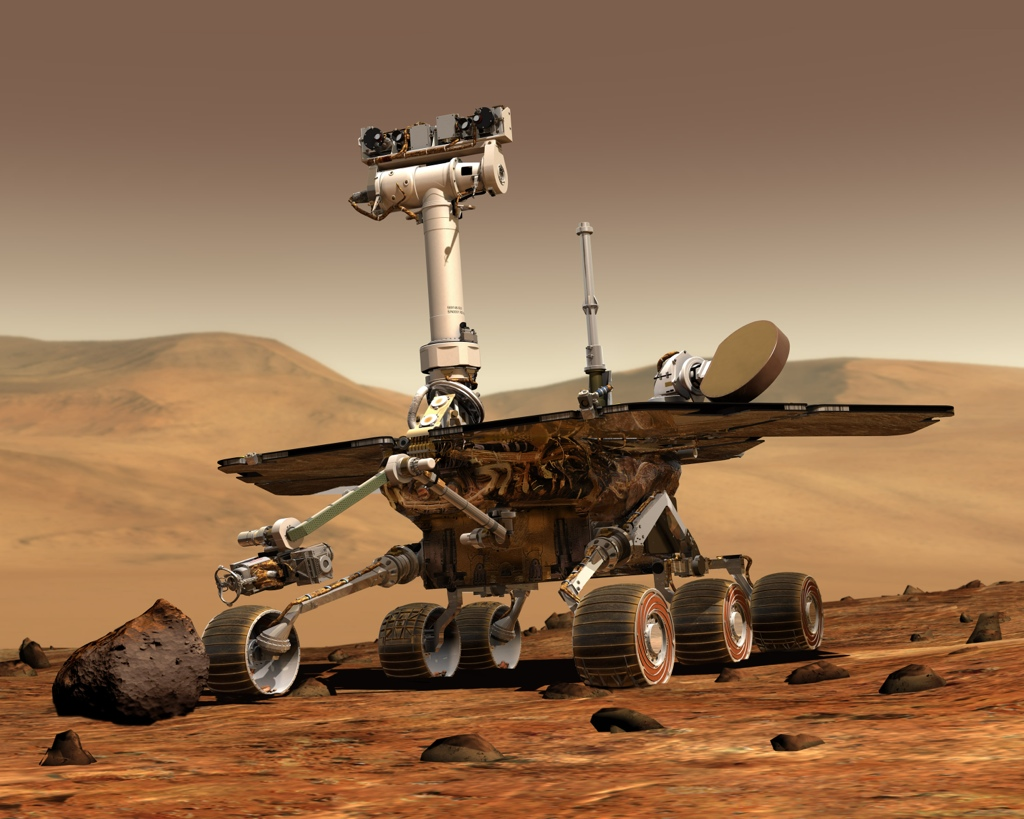
\includegraphics[width=6cm]{images/nasa_rover}
  \caption{Ein Nasa Rover}
  \label{Kap2:NasaRover}
\end{figure}

Man kann sich auch selbst ein Makro für das Einfügen von Bildern schreiben:

\bild{images/modell_point_to_point}{6cm}{Point to Point}

\begin{sidewaysfigure}
 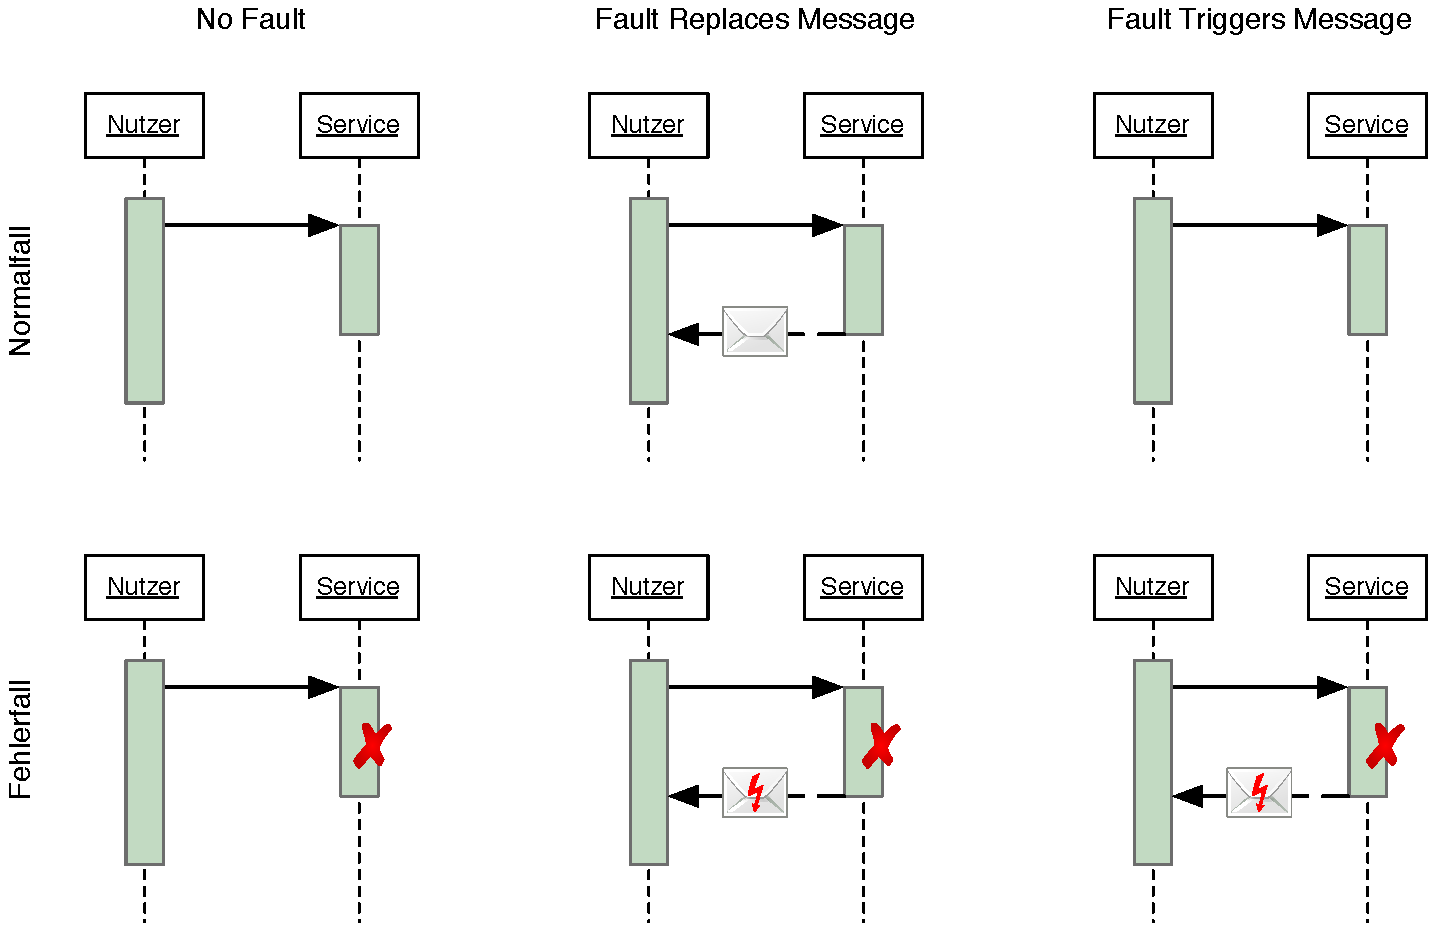
\includegraphics[width=22cm]{images/ws-wsdl20-fehler}
  \caption{Sehr große Grafiken kann man drehen, damit sie auf die Seite passen}
  \label{Kap2:wsdl-fehler}
\end{sidewaysfigure}

\clearpage % Alle Bilder, die bisher kamen ausgeben


\section{Formelsatz}

Eine Formel gefällig? Mitten im Text $a_2 = \sqrt{x^3}$ oder als eigener Absatz (siehe Formel~\ref{Formel}):

\begin{equation}
\begin{bmatrix}
   1 &  4 &  2 \\
   4 &  0 & -3
\end{bmatrix}
        \cdot
\begin{bmatrix}
   1 &  1 &  0 \\
  -2 &  3 &  5 \\
   0 &  1 &  4
\end{bmatrix}
       {=}
\begin{bmatrix}
  -7 &  15 &  28 \\
   4 &   1 & -12
\end{bmatrix}
\label{Formel}
\end{equation}


\section{Sourcecode}

Man kann mit Latex auch ganz toll Sourcecode in den Text aufnehmen.

\subsection{Aus einer Datei}

\lstinputlisting[firstline=2,language=Java,caption={Crypter-Interface},label=lst:CrypterInterface]{\sourcecode/Crypter.java}


\subsection{Inline}

\begin{lstlisting}[language=Java,caption=Methode checkKey()]
    /**
     * Testet den Schlüssel auf Korrektheit: Er muss mindestens die Länge 1
     * haben und darf nur Zeichen von A-Z enthalten.
     *
     * @param key zu testender Schlüssel
     * @throws CrypterException wenn der Schlüssel nicht OK ist.
     */
    protected void checkKey(Key key) throws CrypterException {

        // Passt die Länge?
        if (key.getKey().length == 0) {
            throw new CrypterException("Der Schlüssel muss mindestens " +
                    "ein Zeichen lang sein");
        }

        checkCharacters(key.getKey(), ALPHABET);
    }
\end{lstlisting}


\section{Anforderungen}

Anforderungen im Format des Volere"=Templates (Snowcards) \autocite{Volere} können per Makro eingefügt werden. Das Label wird automatisch mit der Nummer erstellt, d.\,h. Sie können auf die Tabelle mit dieser referenzieren (siehe \autoref{F52}).

Die Abgrenzung von funktionalen und nicht-funktionalen Anforderungen ist nicht immer einfach und bereitet manchen Studierenden Probleme. Als Hilfestellung kann die von der ISO25010 \autocite{ISO25010} zur Verfügung gestellte Liste dienen, siehe \autoref{kapitel3/iso25010}.

\bild{images/iso25010}{14cm}{Qualitätsmodell für Software-Produkte nach ISO25010}

\citeauthor{Bass2003} listen in \autocite{Bass2003} eine ähnliche Liste von Kategorien für nicht-funktionalen Anforderungen auf, die ebenfalls als Richtschnur dienen kann. Diese sind:

\begin{itemize}
  \item \textit{Verfügbarkeit} \textit{(availability)} -- umfasst Zuverlässigkeit (reliability), Robustheit (robustness), Fehlertoleranz (fault tolerance) und Skalierbarkeit (scalability)
  \item \textit{Anpassbarkeit} \textit{(modifiability)}, umfasst Wartbarkeit (maintainability), Verständlichkeit (understandability) und Portabilität (portability).
  \item \textit{Performanz} \textit{(performance)}
  \item \textit{Sicherheit} \textit{(security)}
  \item \textit{Testbarkeit} \textit{(testability)}
  \item \textit{Bedienbarkeit} \textit{(usability)}
\end{itemize}
 % Externe Datei einbinden
\input{chapters/chapter4} % Externe Datei einbinden 
% ------------------------------------------------------------------

\label{lastpage}

% Neue Seite
\cleardoublepage 

% Literaturverzeichnis erzeugen
\begingroup
\cleardoublepage 
\let\clearpage\relax % Fix für leere Seiten (issue #25)
\printbibliography 
\endgroup

% Abkürzungsverzeichnis
\addchap{\frauasabbreviations}
% Die längste Abkürzung kann in die eckigen Klammern
% bei \begin{acronym} geschrieben, um einen hässlichen
% Umbruch zu verhindern
%
% ACHTUNG: Sie müssen die Abkürzungen von Hand alphabetisch
%          sortieren. Das passiert nicht automatisch.
\begin{acronym}[IEEE]
\acro{ABK}{Abkürzung}
\acro{ACM}{Association of Computing Machinery}
\acro{PDF}{Portable Document Format}
\acro{IEEE}{Institute of Electrical and Electronics Engineers}
\acro{ISO}{International Organization for Standardization}
\end{acronym}


% Tabellenverzeichnis erzeugen
\cleardoublepage
\phantomsection
\addcontentsline{toc}{chapter}{\frauaslistoftables}
\listoftables

% Abbildungsverzeichnis erzeugen
\cleardoublepage
\phantomsection
\addcontentsline{toc}{chapter}{\frauaslistoffigures}
\listoffigures

% Listingverzeichnis erzeugen. Wenn Sie keine Listings haben,
% entfernen Sie einfach diesen Teil.
\cleardoublepage
\phantomsection
\addcontentsline{toc}{chapter}{\frauaslistings}
\lstlistoflistings

% Index ausgeben. Wenn Sie keinen Index haben, entfernen Sie einfach
% diesen Teil. Die meisten Abschlussarbeiten haben *keinen* Index.
\cleardoublepage
\phantomsection
\addcontentsline{toc}{chapter}{\frauasindex}
\printindex

% Anhang. Wenn Sie keinen Anhang haben, entfernen Sie einfach
% diesen Teil.
\appendix
\chapter{Erster Anhang}

Hier ein Beispiel für einen Anhang. Der Anhang kann genauso in Kapitel und Unterkapitel unterteilt werden, wie die anderen Teile der Arbeit auch.
 

\end{document}
